\section{Declarative goals and domain properties\label{section:background-goals}}

A \emph{goal} is a prescriptive statement of intent whose satisfaction requires the collaboration of agents forming the system. Unlike goals, \emph{domain properties} are descriptive statement about the environment -- such as physical laws, organizational rules, etc. Goals are structured in AND/OR refinement graphs that show how they contribute to each other~\cite{VanLamsweerde:2000}.

Section~\ref{subsection:background-goals-as-fltl-assertions} formalizes goals and domain properties in fluent linear temporal logic (FLTL). Their integration with state machines and scenarios is discussed in Section~\ref{subsection:background-goals-consistency}. Section~\ref{subsection:background-property-and-tester-automata} then presents how all system traces satisfying (resp. violating) a goal can be specified through a property (resp. a tester) automata, provided that the goal denotes a pure safety property.

\subsection{Properties as FLTL assertions\label{subsection:background-goals-as-fltl-assertions}}

Goals and domain properties can be formalized in Linear Temporal Logic (LTL). Admissible system histories are thereby specified in a declarative and implicit way~\cite{VanLamsweerde:2009}. We will focus on propositional LTL here. In addition to the usual propositional constructs, LTL provides connectives for temporal referencing~\cite{Manna:1992}: 

\begin{itemize}
\item $\circ$ (at the next smallest time unit), 
\item $\diamond$ (some time in the future), 
\item $\square$ (always in the future), 
\item $\rightarrow$ (implies in the current state), 
\item $\Rightarrow$ (always implies), 
\item $\mathcal{U}$ (always in the future until), 
\item $\mathcal{W}$ (always in the future unless)
\end{itemize}

A system history is commonly seen in LTL as a temporal sequence of system states. Atomic LTL propositions then refer to state formulas (as, e.g. in the SPIN model-checker~\cite{Holzmann:1997}). In our event-based setting, a system history will be seen as a trace, that is, a temporal sequence of events. 

To integrate the state-based and event-based paradigms, we will use a flavor of LTL known as Fluent Linear Temporal Logic (FLTL), where atomic propositions are fluents~\cite{Giannakopoulou:2003}. FLTL proves convenient for specifying state-based temporal logic properties over the event-based operational model given by scenarios and state machines. 

For example, the safety goal ``\emph{Doors shall remain closed while the train is moving}'' of our running example can be formalized in terms of the $Moving$ and $DoorsClosed$ fluents, defined in the previous section:
\begin{center}
\artifact{Maintain[DoorsClosed While Moving]} = $\square(Moving \rightarrow DoorsClosed)$
\end{center}

Properties formalized in temporal logic are commonly classified as \emph{liveness} or \emph{safety} properties~\cite{Alpern:1986}. Liveness refers to ``\emph{something good will eventually happen}'' whereas safety refers to  ``\emph{something bad may never happen}''. The thesis will focus on safety properties for the following reasons:
\begin{itemize}
\item Reasoning about liveness requires considering the acceptance of infinite execution traces; this is outside the expressiveness of our LTS characterization and regular languages in general. In contrast, if ``something bad'' happens it must do so after a finite sequence of events, and is irremediable~\cite{Alpern:1986, Giannakopoulou:1999}.
\item The thesis focusses on requirements engineering models. To be realizable by agents, the properties assigned to them must be bounded as \emph{maintain} or \emph{bounded achieve} specifications \cite{Letier:2002}; these correspond to safety properties.  
\end{itemize}

\subsection{Consistency between the behavioral and intentional views\label{subsection:background-goals-consistency}}

Consider a safety property $G$ and a system $\system$. Let $\mathcal{L}^{-}(G)$ denote the set of event traces violating the property and $\mathcal{L}^{+}(G)$ those satisfying it. We discuss how these languages can be captured with automata in the following section.

The system $S$ and the property $G$ are consistent if and only if the following condition holds:
\begin{equation}
\mathcal{L}(Ag_1 \parallel \ldots \parallel Ag_n) \cap \mathcal{L}^{-}(G) = \emptyset
\label{equation:state-machines-and-goals-consistency}
\end{equation}

The above relation requires the system to exclude any trace violating the property. This relation is the one commonly used in model checking, provided that $\mathcal{L}^{-}(G)$ actually amounts to $\mathcal{L}^{+}(\neg G)$ \cite{Clarke:1989}. In other words, $\mathcal{L}^{-}(G)$ actually captures the set of traces satisfying the negation of the safety property.

We also consider consistency rules between goals and scenarios, as follows:
\begin{itemize}
\item Behaviors illustrated in positive scenarios may not violate safety properties. A more formal expression of this depends on the concrete form of scenario specification (scenario collection or hMSC) and on hypotheses about event ordering and weak or strong bMSC synchronization. It is similar to relation (\ref{equation:state-machines-and-goals-consistency}), \emph{mutatis mutandis}.
\item A negative scenario $N$ \emph{illustrates} the violation of a safety property, say $G$, if the following condition holds:
\begin{equation}
\mathcal{L}^{-}(N) \subseteq \mathcal{L}^{-}(G)
\end{equation}
\noindent that is, if the negative traces it defines are among those prescribed by the safety property.
\end{itemize}

\subsection{Property and tester automata\label{subsection:background-property-and-tester-automata}}

For a safety property $G$, the sets of traces $\mathcal{L}^{+}(G)$ and $\mathcal{L}^{-}(G)$ are complement of each other, that is,
\begin{equation}
\mathcal{L}^{+}(G) = \Sigma^{*} \setminus \mathcal{L}^{-}(G)
\end{equation}

Both languages can be specified through standard automata. The one for $\mathcal{L}^{+}(G)$ will be called \emph{property} automaton \cite{Letier:2005} whereas the one for $\mathcal{L}^{-}(G)$ will be called \emph{tester} automaton \cite{Giannakopoulou:2003}. Unlike those references, our characterization here makes use of standard automata instead of LTS.

An example of tester and property automata is given in Fig.~\ref{image:tester-and-property-automata} for the safety goal that requires the doors to remain closed while the train is moving.
\begin{figure}\centering
\scalebox{0.41}{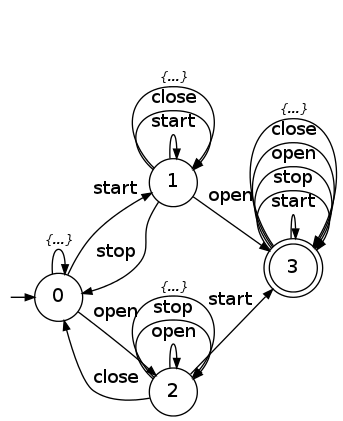
\includegraphics{src/2-framework/images/tester-automaton}}
\scalebox{0.41}{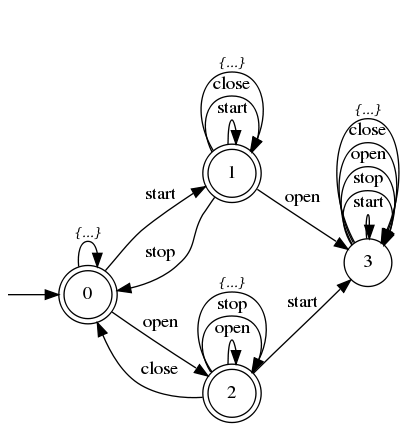
\includegraphics{src/2-framework/images/property-automaton}}
\caption{Tester ($\mathcal{L}^{-}$ at left) and property ($\mathcal{L}^{+}$ at right) automata for \artifact{Maintain[DoorsClosed While Moving]}, as complements of each other.\label{image:tester-and-property-automata}}
\end{figure}

A procedure for computing tester automata in the case of safety properties is given in \cite{Giannakopoulou:2003}. It consists in building a B\"uchi automaton that recognizes all infinite event-based traces that violate the state-based FLTL property. Given a pure safety property, a canonical form for this automaton can been found; the latter is deterministic, has a complete transition function, and a unique sink accepting state reached by all traces violating the property~\cite{Giannakopoulou:2003}.

As tester and property automata are complements of each other, it suffices to flip accepting and non-accepting states of one automaton to obtain the other~\cite{Hopcroft:1979}. A necessary condition, guaranteed by~\cite{Giannakopoulou:2003}, is that they have complete transition functions.

A few remarks are in order here:
\begin{itemize}
\item In the LTSA tool \cite{Magee:1999} and related literature, notably \cite{Giannakopoulou:2003}, a tester LTS with an error state is used instead of the tester automaton presented here. Similarly, the property LTS is sometimes built by removing the error state of the tester LTS \cite{Letier:2008}. 

Our automata variants are better suited here in view of the formalization of inter-model consistency rules expressed in terms of set-theoretic operators on languages.

\item The tester and property automata, together with the procedure for computing them, are always defined ``up to a given alphabet'' or ``under the assumption of a given agent or system''. This is the intended meaning of the transitions labeled ``\emph{\{...\}}" in Fig.~\ref{image:tester-and-property-automata}. The reason is that some temporal properties, in particular those referring to the FLTL \emph{next} operator, are not closed under stuttering~\cite{Lamport:1994}. This means that their satisfaction may be affected by the insertion or removal of unobservable events. Which events are relevant may depend on additional hypotheses about how goals relate to agent behaviors -- e.g, whether they are under the responsibility of a single agent or are properties to be met by the global system. Fixing those ``relevant events'' by filling the ``\emph{\{...\}}" placeholder is required for meeting the temporal logic semantics when composing tester and property automata. 

For simplicity in the thesis, we will consider that safety properties must be met by the global system. Therefore, the relevant events are the alphabet of the whole system, say $\Sigma$. A placeholder then must be replaced by a transition for each event in $\Sigma$ except those already labeling an outgoing transition from the same state.
\end{itemize}
